\documentclass{beamer}

\usepackage{tikz}

\title{Parasites in Structural and Dynamical models of Food Webs}
\author{Nick Kappler}
\date{\today}


\begin{document}
\frame{\titlepage}

\section[Outline]{}
\frame{\tableofcontents}

\section{Motivation}

\begin{frame}
\frametitle{Parasitism in Food Webs}
\begin{itemize}[<+->]
\item  Underrepresented
\item  Novel, complex, and specific
\item  Place in Food Webs
\end{itemize}
\end{frame}

\begin{frame}
\frametitle{Past Work}
\begin{itemize}[<+->]
\item  Effects of Adding Parasites %\footnote{\tiny\bibentry{Dunne2013}}
\item  Importance of Body Size Ratios %\footnote{\tiny\bibentry{Brose2006}}
\item  An Inverse Niche Model %\footnote{\tiny\bibentry{Warren2010}}
\item  Why?
\end{itemize}
\end{frame}

\begin{frame}
\frametitle{Research Goals}
\begin{itemize}[<+->]
\item Niche Model vs. Inverse Niche Model(s)
\item  Dynamical Simulations
\item  Concommitant (Incidental) Predation
\end{itemize}
\only<3>{
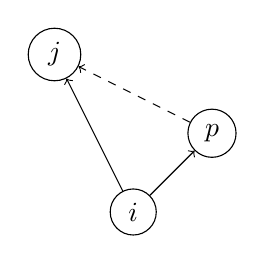
\begin{tikzpicture}
\node[draw,circle] at (0,0) (j) {$j$};
\node[draw,circle] at (1,-2) (i) {$i$};
\node[draw,circle] at (2,-1) (p) {$p$};
\draw[->] (i)--(j);
\draw[->] (i)--(p);
\draw[->,dashed] (p)--(j);
\end{tikzpicture}
}
\end{frame}


\subsection{Niche Model}

\subsection{ATN Model}

\subsection{Small Consumers}

\subsection{Coupling ATN + Niche Model}

\section{Niche Model Additions}

\subsection{Proposed Models}

\subsection{Results}

\section{ATN Additions}

\subsection{Proposed Models}

\subsection{Results}

\section{Conclusions}

\section{Future Work}
\end{document}
